% Figure 3 - The pairing machinery (theory section), single-column (86 mm).
% Three flat, technical panels:
%   (a) two-band charge sharing (SSH4-derived): alkali sp_z band descends
%       through E_F as the gallery opens; splitting set by transferred charge dq.
%   (b) parity selection: gallery-midplane mirror, sodium displacement delta odd;
%       linear e-ph vertex g1=0 (crossed out), quadratic 1/2 chi delta^2 allowed.
%   (c) quantized double well: tunnelling doublet E0,E1 and E2; the pairing
%       boson is the overtone hbar Omega = E2 - E0 (E0->E1 forbidden by parity).
%
% Design note: placed at \columnwidth (86 mm); drawn at small natural width with
% >= \footnotesize fonts and minimal text.  Build:  pdflatex fig3_model.tex
\documentclass[10pt,border=2pt]{standalone}
\usepackage{tikz}
\usepackage{amsmath}
\usepackage{mathptmx}
\usetikzlibrary{arrows.meta,positioning,decorations.pathreplacing,
                decorations.pathmorphing,decorations.markings,calc}

% ---- palette (flat, physics-encoding) ---------------------------------------
\definecolor{ink}{HTML}{0B0B0B}
\definecolor{sec}{HTML}{52514E}
\definecolor{mut}{HTML}{898781}
\definecolor{na}{HTML}{E58A00}       % alkali / sodium
\definecolor{nadk}{HTML}{9A5B00}
\definecolor{egas}{HTML}{2A78D6}     % electron / CoO2 band / levels
\definecolor{coox}{HTML}{4A5A63}     % CoO2 band
\definecolor{crit}{HTML}{C23A38}     % forbidden (parity)
\definecolor{good}{HTML}{0C8A2E}     % allowed

\begin{document}
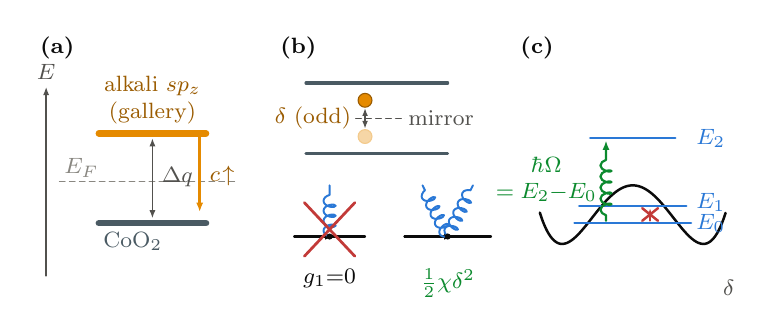
\begin{tikzpicture}[x=1cm,y=1cm,line join=round,line cap=round,
    ph/.style={egas,line width=0.7pt,decorate,             % phonon (coil)
       decoration={coil,aspect=0.55,segment length=3.6pt,amplitude=2.2pt}},
    eline/.style={ink,line width=0.8pt,                     % electron line
       postaction={decorate,decoration={markings,
         mark=at position 0.56 with {\arrow[line width=0.6pt]{Latex[length=3.2pt]}}}}},
    band/.style={line width=2.4pt},
    lvl/.style={egas,line width=0.9pt},
  ]

  \def\Q{3.05}          % panel pitch
  \def\panlab#1#2{\node[ink,font=\footnotesize\bfseries,anchor=south west]
     at (#1,2.98) {#2};}

  % ================================================================= PANEL (a)
  % Two-band charge sharing.  Alkali sp_z band (upper) descends through E_F and
  % donates dq to the CoO2 band (lower); the band splitting is set by dq.
  \begin{scope}[shift={(0,0)}]
    \panlab{-0.15}{(a)}
    % energy axis
    \draw[sec,line width=0.5pt,-{Latex[length=3pt]}] (0.05,0.35) -- (0.05,2.75);
    \node[sec,font=\footnotesize,anchor=south] at (0.05,2.72) {$E$};
    % Fermi level (label at left, above the line)
    \draw[mut,line width=0.5pt,dashed,dash pattern=on 2pt off 1.6pt]
      (0.22,1.55) -- (2.48,1.55);
    \node[mut,font=\footnotesize,anchor=south west,inner sep=1pt] at (0.24,1.56) {$E_F$};
    % alkali band (above E_F)
    \draw[band,na] (0.72,2.16) -- (2.08,2.16);
    \node[nadk,font=\footnotesize,anchor=south,align=center,inner sep=1pt]
      at (1.4,2.24) {alkali $sp_z$\\(gallery)};
    % CoO2 band (occupied, below E_F)
    \draw[band,coox] (0.72,1.02) -- (2.08,1.02);
    \node[coox,font=\footnotesize,anchor=north,inner sep=1pt] at (1.15,0.94) {CoO$_2$};
    % splitting = transferred charge dq (centred double arrow)
    \draw[sec,line width=0.6pt,{Latex[length=3pt]}-{Latex[length=3pt]}]
      (1.4,2.10) -- (1.4,1.08);
    \node[sec,font=\footnotesize,anchor=west,inner sep=1.5pt] at (1.46,1.6) {$\Delta q$};
    % alkali band descends through E_F as the gallery opens (c increases)
    \draw[na,line width=0.9pt,-{Latex[length=3.4pt]}] (2.0,2.12) -- (2.0,1.16);
    \node[nadk,font=\footnotesize,anchor=west,inner sep=1.2pt] at (2.08,1.62) {$c\!\uparrow$};
  \end{scope}

  % ================================================================= PANEL (b)
  % Parity selection.  Midplane mirror; sodium displacement delta odd under it.
  % Linear vertex g1 = 0 (crossed); quadratic 1/2 chi delta^2 allowed.
  \begin{scope}[shift={(\Q,0)}]
    \panlab{-0.15}{(b)}
    % --- gallery-midplane mirror + odd (vertical, c-axis) displacement ---
    % two thin horizontal CoO2 sheets with a dashed midplane (the mirror)
    % between them; the sodium rattles VERTICALLY toward one sheet or the other.
    \draw[coox,line width=1.1pt] (0.30,2.80) -- (2.10,2.80);   % upper CoO2 sheet
    \draw[coox,line width=1.1pt] (0.30,1.90) -- (2.10,1.90);   % lower CoO2 sheet
    \draw[sec,line width=0.5pt,dashed,dash pattern=on 2pt off 1.6pt]
      (0.30,2.35) -- (2.10,2.35);
    % ion ghosted above (+delta) and below (-delta) the midplane
    \node[circle,draw=nadk,fill=na,line width=0.4pt,minimum size=5pt,
      inner sep=0pt] at (1.05,2.58) {};
    \node[circle,draw=na!45!white,fill=na!35,line width=0.4pt,minimum size=5pt,
      inner sep=0pt] at (1.05,2.12) {};
    % vertical double-headed arrow : delta (odd)
    \draw[sec,line width=0.5pt,{Latex[length=2.8pt]}-{Latex[length=2.8pt]}]
      (1.05,2.48) -- (1.05,2.22);
    % labels sit on the midplane; white fill masks the dashed line behind them
    \node[nadk,font=\footnotesize,anchor=east,inner sep=1.2pt,fill=white] at (0.92,2.35)
      {$\delta$ (odd)};
    \node[sec,font=\footnotesize,anchor=west,inner sep=1.2pt,fill=white] at (1.55,2.35)
      {mirror};
    % --- two vertices (lower) ---
    % linear vertex : forbidden
    \draw[eline] (0.15,0.85) -- (1.05,0.85);
    \draw[ph] (0.6,0.85) -- (0.6,1.5);
    \fill[ink] (0.6,0.85) circle (1.1pt);
    \draw[crit,line width=1.0pt] (0.28,0.6) -- (0.92,1.28);
    \draw[crit,line width=1.0pt] (0.28,1.28) -- (0.92,0.6);
    \node[ink,font=\footnotesize,anchor=north,align=center,inner sep=1.5pt]
      at (0.6,0.5) {$g_1{=}0$};
    % quadratic vertex : allowed (two phonon lines)
    \draw[eline] (1.55,0.85) -- (2.65,0.85);
    \draw[ph] (2.1,0.85) -- (1.78,1.5);
    \draw[ph] (2.1,0.85) -- (2.42,1.5);
    \fill[ink] (2.1,0.85) circle (1.1pt);
    \node[good,font=\footnotesize,anchor=north,align=center,inner sep=1.5pt]
      at (2.1,0.5) {$\tfrac12\chi\delta^2$};
  \end{scope}

  % ================================================================= PANEL (c)
  % Quantized double well: tunnelling doublet E0,E1 (near-degenerate) and E2.
  % Pairing boson = overtone hbar Omega = E2 - E0.  E0->E1 forbidden (parity).
  \begin{scope}[shift={(2*\Q,0)}]
    \panlab{-0.15}{(c)}
    % double-well curve  V(delta)
    \draw[ink,line width=0.9pt,smooth,domain=-1.18:1.18,samples=90]
      plot ({1.4+\x},{0.55+0.95+(-1.85*\x*\x+1.15*\x*\x*\x*\x)});
    \node[sec,font=\footnotesize,anchor=north] at (2.62,0.42) {$\delta$};
    % levels (right-labelled)
    \draw[lvl] (0.66,1.02) -- (2.14,1.02);            % E0
    \node[egas,font=\footnotesize,anchor=west,inner sep=1.2pt] at (2.16,1.02){$E_0$};
    \draw[lvl] (0.72,1.24) -- (2.08,1.24);            % E1 (near-degenerate)
    \node[egas,font=\footnotesize,anchor=west,inner sep=1.2pt] at (2.16,1.28){$E_1$};
    \draw[lvl] (0.86,2.10) -- (1.94,2.10);            % E2 (above barrier)
    \node[egas,font=\footnotesize,anchor=west,inner sep=1.2pt] at (2.16,2.10){$E_2$};
    % pairing boson : overtone hbar Omega = E2 - E0  (wavy up-arrow)
    \draw[good,line width=0.8pt,decorate,
       decoration={coil,aspect=0.5,segment length=4pt,amplitude=2pt,
                   pre length=2pt,post length=4pt},-{Latex[length=3.4pt]}]
      (1.06,1.05) -- (1.06,2.07);
    \node[good,font=\footnotesize,anchor=east,align=center,inner sep=1.5pt]
      at (1.0,1.58) {$\hbar\Omega$\\$=E_2{-}E_0$};
    % E0 -> E1 forbidden by parity (crossed short arrow)
    \draw[crit,line width=0.6pt,-{Latex[length=2.6pt]}] (1.62,1.05) -- (1.62,1.21);
    \draw[crit,line width=0.9pt] (1.52,1.05) -- (1.72,1.21);
    \draw[crit,line width=0.9pt] (1.52,1.21) -- (1.72,1.05);
  \end{scope}

\end{tikzpicture}
\end{document}
